
Figure~\ref{code:language:message} shows the first LM program, a message routing
program that simulates message transmission through a network of nodes. In
lines~\ref{line:language:message_pred1}-\ref{line:language:message_pred2} we
declare the predicates used in the program's rules. Note that the first argument
of every predicate must be typed as \code{node} because the first argument
indicates where the node lives in the graph. Predicate \code{edge} is a
\emph{persistent predicate} while \code{message} and \code{processed} are
\emph{linear predicates}. Persistent predicates model facts that are never
retracted from the database, while linear predicates model linear facts which
are retracted when used in rules. To improve readability of LM rules, persistent
predicates are preceded with a \code{!} symbol. Predicate \code{edge} represents
the connections between nodes, predicate \code{message} contains the message
content and the route list, and predicate \code{processed} keeps count of the
number of messages routed at each node. Along with the type, a predicate
argument can also be named (see \code{Neighbor} and \code{Content}) for
documentation purposes.

\begin{figure}[h!]
\begin{Verbatim}[numbers=left,commandchars=\*\{\},fontsize=\codesize]
type edge(node, node Neighbor).*label{line:language:message_pred1}
type linear message(node, string Content, list node Routing).
type linear processed(node, int Total).*label{line:language:message_pred2}

!edge(A, B),*label{line:language:message_first1}
message(A, Content, [B | L]),
processed(A, N)
   -o message(B, Content, L),
      processed(A, N + 1).*label{line:language:message_first2}

message(A, Content, []),*label{line:language:message_second1}
processed(A, N)
   -o processed(A, N + 1).*label{line:language:message_second2}

!edge(@1, @2). !edge(@2, @3). !edge(@3, @4). !edge(@1, @3).*label{line:language:message_axioms}
processed(@1, 0). processed(@2, 0). processed(@3, 0). processed(@4, 0).
message(@1, "hello world", [@3, @4]).*label{line:language:message_message}
\end{Verbatim}
\caption{Code for routing messages in a graph. There is only one message ("hello
world") to route through nodes \code{@3} and \code{@4}.}
\label{code:language:message}
\end{figure}

The message routing program in Fig.~\ref{code:language:message} implements two
rules in
lines~\ref{line:language:message_first1}-\ref{line:language:message_first2}. An
LM rule has the form $L_1, \cdots, L_n \mathtt{-o} \; R_1, \cdots, R_m$, where
$L_1, \cdots, L_n$ is the \emph{left-hand side}~(LHS) of the rule while $R_1,
\cdots, R_m$ is \emph{right-hand side}~(RHS) of the rule. The meaning of a rule
is then as follows: if facts $L_1, \cdots, L_n$ are present in the database then
retract facts $L_i$ that are linear facts and derive the facts $R_1, \cdots,
R_m$ from the RHS. Note that in all the rules, the LHS of each rule uses facts
from the same node (in this particular case, \code{A}), but the rule's RHS may
derive facts in other nodes (\code{B} in the first rule) because a node variable
was instantiated in the LHS.

The first rule
(lines~\ref{line:language:message_first1}-\ref{line:language:message_first2})
grabs the head node in the route list (third argument of \code{message}) using
the syntax \code{[B | L]} and ensures that a communication edge exists (through
\code{edge(A,~B)}). We increase the number of processed messages by consuming
\code{processed(A,~N)} and deriving \code{processed(A,~N~+~1)}.  When the route
list is empty, the message has reached its destination and thus it is consumed
(rule in lines
\ref{line:language:message_first1}-\ref{line:language:message_first2}).

The initial facts of the program are declared in
lines~\ref{line:language:message_axioms}-\ref{line:language:message_message}.
The \code{edge(a, b)} facts describe the structure of the graph, where node
\code{a} has a direct connection with node \code{b}. Node literals are
represented using the syntax \code{@N}, where \code{N} is an non-negative
number. In line~\ref{line:language:message_message} we declare the message that
needs to be routed and has the content \code{"hello world"} and a route list
with the nodes \code{@3} and \code{@4}.

In Fig.~\ref{fig:message_trace} we present an execution trace of the message
routing program. The database is represented as a graph structure where the
edges represent the \code{edge} initial facts. To simplify the figure, we
dropped the first argument of each fact since the first argument corresponds to
the node where the fact is placed. In Fig.~\ref{fig:message_trace}~(a) the
database is initialized with the program's initial facts. Note that the initial
\code{message} fact is instantiated at node \code{@1}. After applying rule 1, we
get the database represented in Fig.~\ref{fig:message_trace}~(b), where the
message has been derived at node \code{@3}. After applying rule 1 again, the
message is then routed to node \code{@4} (Fig.~\ref{fig:message_trace}~(c))
where it will be consumed (Fig.~\ref{fig:message_trace}~(d)).

\newcommand{\visitsize}{0.38}

\begin{figure}[h]
        \centering
        \begin{subfigure}[b]{\visitsize\textwidth}
                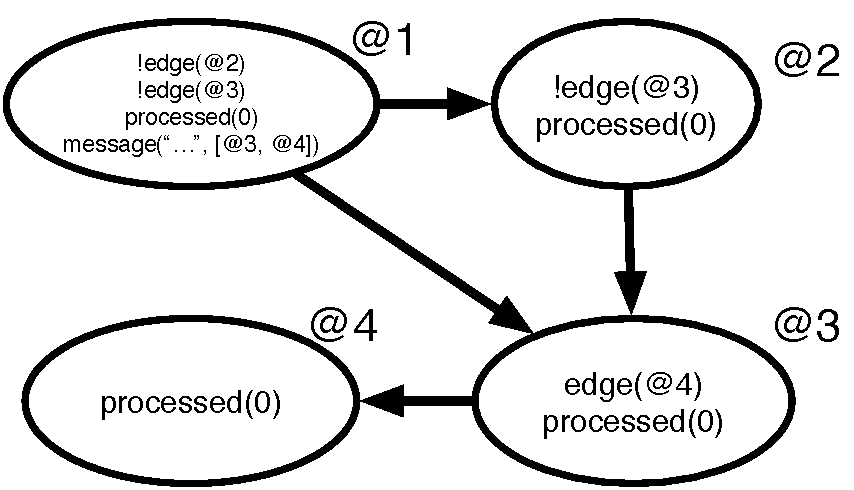
\includegraphics[width=\textwidth]{figures/message/message_trace1}
                \caption{Initial database.}
                \label{fig:message_trace1}
        \end{subfigure}%
        ~
        \begin{subfigure}[b]{\visitsize\textwidth}
                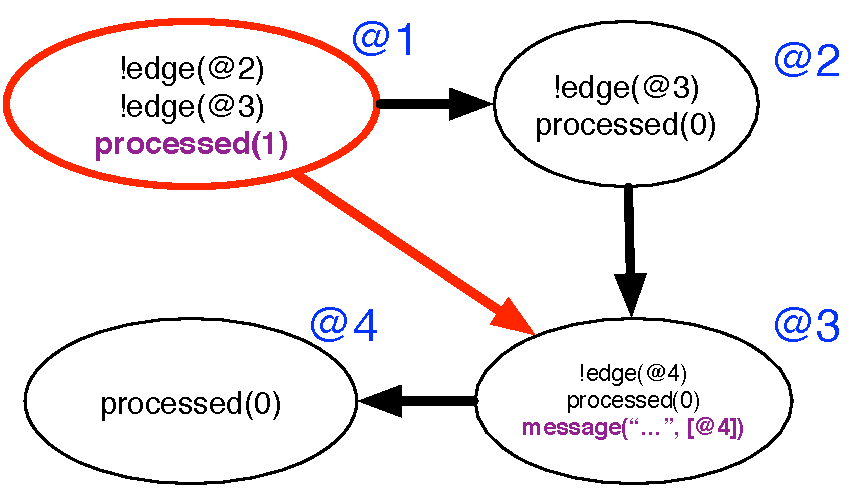
\includegraphics[width=\textwidth]{figures/message/message_trace2}
                \caption{After applying rule 1 at node \code{@1}.}
                \label{fig:message_trace2}
        \end{subfigure}\\
        \begin{subfigure}[b]{\visitsize\textwidth}
                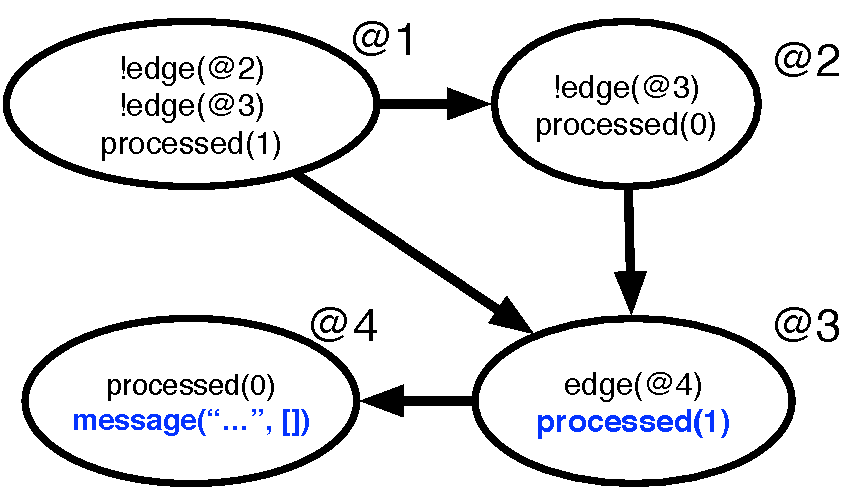
\includegraphics[width=\textwidth]{figures/message/message_trace3}
                \caption{After applying rule 1 at node \code{@3}.}
                \label{fig:message_trace3}
        \end{subfigure}%
        ~
        \begin{subfigure}[b]{\visitsize\textwidth}
                  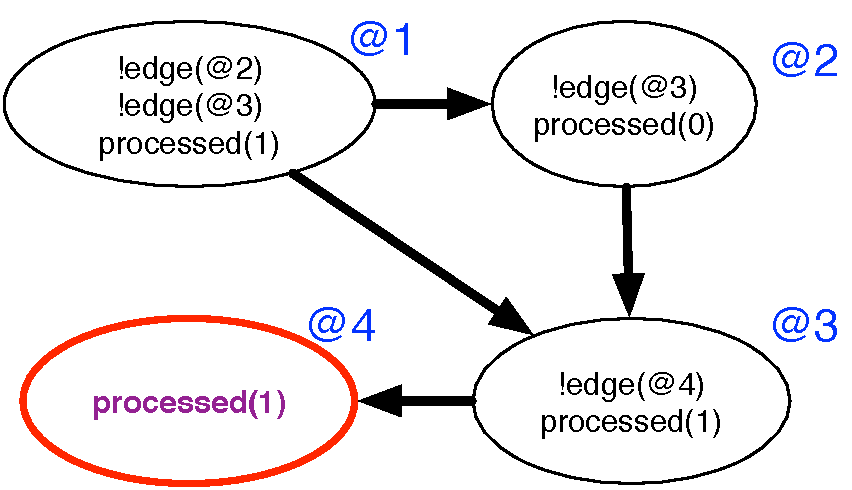
\includegraphics[width=\textwidth]{figures/message/message_trace4}
                  \caption{After applying rule 2 (nodes \code{@4}).}
                  \label{fig:message_trace4}
          \end{subfigure}
        \caption{An execution trace for the message program. The message "hello
        world" travels from node \code{@1} to node \code{@4}.}\label{fig:message_trace}
\end{figure}

The attentive reader will wonder how much concurrency is available in this
particular routing implementation. For a single message, there is not much
concurrency because the message follows a pre-determined path and it travels
from node to node. However, concurrency arises when the program needs to route
multiple messages. The amount of concurrency is then dependent on the messages
routing lists being non-overlapping. If messages travel in different paths, then
there is more concurrency because more nodes are routing messages at the same
time.
